%%%%%%%%%%%%%%%%%%%%%%%%%%%%%%%%%%%%%%%%%%%%%%%%%%%%%%%%%%%%%%%%%%
%%%%%%%% ICML 2016 EXAMPLE LATEX SUBMISSION FILE %%%%%%%%%%%%%%%%%
%%%%%%%%%%%%%%%%%%%%%%%%%%%%%%%%%%%%%%%%%%%%%%%%%%%%%%%%%%%%%%%%%%

% Use the following line _only_ if you're still using LaTeX 2.09.
%\documentstyle[icml2016,epsf,natbib]{article}
% If you rely on Latex2e packages, like most moden people use this:
\documentclass{article}

% use Times
\usepackage{times}
% For figures
\usepackage{graphicx} % more modern
%\usepackage{epsfig} % less modern
%\usepackage{subfigure} 

% For citations
\usepackage{natbib}


% For algorithms

% As of 2011, we use the hyperref package to produce hyperlinks in the
% resulting PDF.  If this breaks your system, please commend out the
% following usepackage line and replace \usepackage{icml2016} with
% \usepackage[nohyperref]{icml2016} above.
\usepackage{hyperref}

% Packages hyperref and algorithmic misbehave sometimes.  We can fix
% this with the following command.
\newcommand{\theHalgorithm}{\arabic{algorithm}}

% Employ the following version of the ``usepackage'' statement for
% submitting the draft version of the paper for review.  This will set
% the note in the first column to ``Under review.  Do not distribute.''
\usepackage{icml2016} 

% Employ this version of the ``usepackage'' statement after the paper has
% been accepted, when creating the final version.  This will set the
% note in the first column to ``Proceedings of the...''
%\usepackage[accepted]{icml2016}

\usepackage{algorithm}
\usepackage{algorithmic}

\usepackage{caption}
%\usepackage{subcaption}
\usepackage{mathptmx}
\usepackage{amsmath}
\usepackage{amssymb}

\usepackage{subcaption}

\newcommand{\w}{w}
\newcommand{\z}{z}
\newcommand{\pfcomment}[1]{{\color{red} PF: #1}}
\newcommand{\sigmatilde}{\tilde{\sigma}}
\newcommand\numberthis{\addtocounter{equation}{1}\tag{\theequation}}

\newtheorem{lemma}{Lemma}
\renewcommand{\thelemma}{\arabic{lemma}}


% The \icmltitle you define below is probably too long as a header.
% Therefore, a short form for the running title is supplied here:
\icmltitlerunning{Stratified Bayesian Optimization}


\begin{document} 

\twocolumn[
\icmltitle{Stratified Bayesian Optimization}

% It is OKAY to include author information, even for blind
% submissions: the style file will automatically remove it for you
% unless you've provided the [accepted] option to the icml2016
% package.
\icmlauthor{Saul Toscano-Palmerin}{st684@cornell.edu}

\icmlauthor{Peter I. Frazier}{pf98@cornell.edu}
\icmladdress{Cornell University,
            257 Rhodes Hall, Ithaca, NY 14853, USA}

% You may provide any keywords that you 
% find helpful for describing your paper; these are used to populate 
% the "keywords" metadata in the PDF but will not be shown in the document
\icmlkeywords{Bayesian, optimization}

\vskip 0.3in
]

%%4-6 sentences long
\begin{abstract} 
We consider derivative-free black-box global optimization of expensive noisy functions,
when most of the randomness in the objective is produced
by a few influential scalar random inputs. We present a new Bayesian global
optimization algorithm, called Stratified Bayesian Optimization (SBO), which uses
this strong dependence to improve performance. Our algorithm is similar in spirit
to stratification, a classical technique from simulation, which uses strong
dependence on a categorical representation of the random input to reduce
variance. We demonstrate in numerical experiments that SBO outperforms a
Bayesian optimization benchmark that does not take advantage of this dependence.
\end{abstract} 


\section{Introduction} 
We consider derivative-free black-box global optimization of expensive noisy functions,
\begin{equation}
\max_{x\in A\subset\mathbb{R}^{n}}\mathbb{E}\left[f\left(x,\w,\z \right)\right],
\label{eq:goal}
\end{equation}
where the expectation is taken over $\z\in\mathbb{R}^{d_1}$ and $\w\in\mathbb{R}^{d_2}$, which have some joint probability density $p$, $A$ is a simple compact set (e.g., a hyperrectangle, or a simplex), and we can directly observe only $f(x,\w,\z)$ at some collection of chosen or sampled $x,\w,\z$, and not its expectation, or the derivative of this expectation.
We suppose that $f$ has no special structural properties, e.g., concavity, or linearity, that we can exploit to solve this problem, making it a ``black blox.''
We also suppose that evaluating $f$ is costly or time-consuming, making these evaluations ``expensive'', severely limiting the number of evaluations we may perform.  This typically occurs because each evaluation requires running a complex PDE-based or discrete-event simulation, or requires training a machine learning algorithm on a large dataset.
When $f$ comes from a discrete-event simulation, this problem is also often called ``simulation optimization.''

Bayesian optimization is a popular class of techniques for solving this problem, originating with the seminal paper \cite{kushner}, and enjoying early contributions from \cite{Mockus:1978,Mockus:1989}. This class of techniques was popularized in the 1990s by the introduction in \cite{jones1998efficient} of the most well-known Bayesian optimization method, Efficient Global Optimization (EGO), relying on earlier ideas from \cite{Mockus:1989}. Recently the machine learning community has devoted considerable interest and effort to Bayesian optimization for its applications to tuning computationally intensive machine learning models, as in, e.g., \cite{snoek2012practical}. Textbooks and surveys on Bayesian optimization include \cite{forrester2008engineering,brochu2010tutorial}.

Most work on Bayesian optimization assumes we can observe the objective function directly without noise, but a substantial number of papers, e.g. \cite{villemonteix2009informational,huang2006global,scott2011correlated,brochu2010tutorial}, do allow noise and thus consider the problem \eqref{eq:goal}. These methods all build a statistical model (usually using Gaussian processes) of the function $x \mapsto G(x) := \mathbb{E}[f(x,\w,\z)]$ using noisy observations, and then use an acquisition criterion, typically expected improvement or probability of improvement \cite{brochu2010tutorial}, to decide where to sample next.

Existing work from Bayesian optimization for solving \eqref{eq:goal} rely on noisy evaluations in which $\w$ and $\z$ are drawn iid from their governing joint probability distribution $p$, and then $f(x,\w,\z)$ is observed.
However, in many applications, we have the ability to choose not just $x$, but $\w$ as well, simulating the remaining components $\z$ conditioning on these values.
(The choice of which random inputs to include in $\w$ and which in $\z$ was arbitrary above, but will be assumed below to accommodate this distinction.)
For example, in a queuing simulation, we can simulate the individual arrival times of customers $\z$ conditioning on the overall number of arrivals $\w$. We explore this in more detail in the numerical experiments. This ability to simulate random inputs given the value of some of their values is widely used in stratified sampling to estimate expectations with better precision \cite{glasserman2003monte}. 

%\pfcomment{Note: should explain that w is low dimensional and conveys a lot of information about f(x,w,z).  Should give an example to articulate this.  In an extreme case, f(x,w,z) doesn't depend on z.}

This ability suggests the rephrasing of problem \eqref{eq:goal} into the equivalent problem
\begin{equation}
\max_{x\in A\subset\mathbb{R}^{n}}\mathbb{E}\left[F\left(x,\w\right)\right]
\label{eq:strata}
\end{equation} 
where $F\left(x,\w\right):=\mathbb{E}\left[f\left(x,\w,\z\right)\mid \w\right]$,
and the problems are equivalent because $\mathbb{E}[F(x,\w)]=\mathbb{E}\left[f\left(x,\w,\z\right)\right] = G(x)$.

% Here, $\w$ is low dimensional and conveys a lot of information about $f(x,w,z)$. There are many problems with this framework, for example, suppose $f$ is the number of people who did not get a bed in a hospital, then $f$ depends strongly on the overall number of arrival, but not on the individual arrival times of customers. In an extreme case, $f(x,w,z)$ does not depend on $\z$. 

This equivalent formulation suggests that standard approaches to Bayesian optimization are wasteful from a statistical point of view, as they do not use past observations $\w$ to learn $G(x) = \mathbb{E}[F(x,\w)]$, treating $\w$ only as an unobservable source of noise.  Instead, one can use Bayesian quadrature \cite{o1991bayes}, which builds a Gaussian process model of the function $F(x,\w)$ using past observations of $x,\w,f(x,\w,\z)$, and then uses the known relationship $G(x) = \int F(x,w) p(w)\,dw$ (where we assume $p(w):=\int p(\w,\z)\,d\z$ is known in closed form) to imply a second Gaussian process model on $G(x)$.
%\pfcomment{Indeed, when one compares the posterior variance on E[F(x,\w)] under the two approaches, the posterior variance obtained using Bayesian quadrature is smaller.}

Using this ability, we develop an algorithm in this paper, called stratified Bayesian optimization (SBO), which chooses not just the $x$ at which to evaluate $f(x,\w,\z)$, but also the $\w$.  It chooses these using an acquisition function discussed below, which is based on a value-of-information \cite{Ho66} calculation, and has a one-step Bayes-optimality property.  It then samples $\z$ from its conditional distribution given $\w$, and uses the resulting observation within a Bayesian quadrature framework to update its Gaussian process posterior on both $(x,\w)\mapsto F(x,\w)$ and $x\mapsto \mathbb{E}[F(x,\w)]$.  By using more information, we make our statistical model more powerful, and allow our optimization framework to provide better answers with fewer samples.

This approach is similar in spirit to stratified sampling \cite{glasserman2003monte}, where our goal is to estimate $G(x) = E[F(x,\w)]=E[f(x,\w,\z)]$ (for a fixed $x$, as this literature does not consider variation in $x$) and we choose which values of $\w$ at which to sample rather than sampling them from their marginal distribution, and then compensate for this choice via a known relationship between $F(x,\w)$ and $G(x)$ to obtain lower variance estimates.

% This equivalent formulation suggests that, rather than carefully choosing just $x$ and letting $\w$ be chosen from its marginal distribution, we may carefully choose both $x$ and $\w$, and build a statistical model not of $x\mapsto \mathbb{E}[F(x,\w)]$, but of 

% Since we can only observe $f$, we can only have noisy observations of $F$. This suggests to have a metamodel not only on $f$, but also on $F$. This allows us to choose $x$ and $\w$ to get noisy observations of $F$. This has the advantage of learning faster the objective function. In more detail, we place a Gaussian process (GP) prior on $F$, and then we use Bayesian quadrature \cite{o1991bayes} to also have a Gaussian process on its expectation. This method allows us to make inferences about the value of the expectation of $F$. We then update these priors when we have new observations, and this reduces our uncertainty about the value of $F$ and its expectation. 
 %Specifically we use the empirical mean to estimate its value. So, for each pair x,w1 %we simulate a batch of samples z. This assumption makes sense because of the central %limit theorem. 

To decide how to choose $x$ and $\w$, we use a decision-theoretic approach which models the utility that results from solutions to the optimization problem \eqref{eq:strata}.  We then find the pair of values ($x,\w$) at which to sample that maximizes the expected utility of the final solution, under the assumption, made for tractability, that we may take only one additional sample.  Thus, our SBO algorithm is optimal in a decision-theoretic sense, in a one-step setting.

This one-step decision-theoretic approach follows the development of acquisition functions designed for other settings.  In more traditional Bayesian optimization problems, the well-known expected improvement acquisition function \cite{Mockus:1989,jones1998efficient} has this optimality property when observations are noise-free and the final solution must be taken from previously evaluated solutions \cite{Frazier:bayesianOpt}, and the knowledge-gradient method \cite{frazier2009knowledge,scott2011correlated} has this optimality property when the final solution is not restricted to be a previously evaluated solution, in both the noisy and noise-free setting.

% The first contribution of this work is to provide a new method, called stratified Bayesian optimization (SBO), for the problem \eqref{eq:goal} when we are able to draw samples from $f(x,\w,\z)$ conditioning on $x$ and $\w$. 

% We demonstrate that this method outperforms standard Bayesian optimization in this setting. 

Our current approach significantly generalizes \cite{Xie:2012}, which developed a similar method, but did not allow for the inclusion of unmodeled random inputs $\z$, instead requiring all inputs to be included and modeled statistically in $\w$.  This introduces a heavy computational and statistical burden when dealing with problems in which the combined dimension of $\w$ and $\z$ is large, such as queuing problems and many other problems from engineering, significantly limiting its applicability.

% built a Gaussian process over the function $(x,\w,\z)\mapsto f(x,\w,\z)$.  Adding $\z$ to the set of variables on which the statistical model is based, and over which the value of information is optimized, adds significant computational complexity to the approach.  

% This makes this previous method computationally infeasible for problems such as queuing control, where the dimension of $\z$ is large, even though the SBO approach that we present here may be profitably applied since $\w$ is small and the conditional variance of $f(x,\w,\z)$ given $\w$ is small.

% than just the dependence of its thus essentially requiring that $\z$ be removed and all components placed into $\w$.  In problems such as queuing control problems, where the dimension of $\w,\z)$ is large, this approach is computationally infeasible because it requires modeling a high-dimensional function, and, more significantly, optimizing the value of information criterion over 


This paper is organized as follows: In $\mathsection$\ref{model}, we present the statistical model used for the problem. In $\mathsection$\ref{SBO},
we present the SBO algorithm. In $\mathsection$\ref{SBO}, we briefly give the main ideas of the computation of the value of information and its derivative. 
In $\mathsection$\ref{experiments}, we present two numerical experiments. In $\mathsection$\ref{conclusion}, we conclude.


% \pfcomment{We should say this somewhere, and then use it through the introduction:
% We define the objective function as $G\left(x\right):=\int F\left(x,\w\right)dp\left(\w\right)$.}



% We consider a continuous function $f:\mathbb{R}^{n}\times\mathbb{R}^{d}\rightarrow\mathbb{R}$ and a probability space $\left(\mathbb{R}^{d},\mathcal{F},P\right)$. We suppose that each evaluation of this function has a cost.
% We denote the joint pdf of $\omega=\left(\w,\z\right)\in\mathbb{R}^{d}=\mathbb{R}^{d_{1}}\times\mathbb{R}^{d_{2}}$
% with $d_{1}\ll d_{2}$ by $p\left(\w,\z\right)$,
% which is assumed known.

% Our goal is to solve
% \begin{equation*}
% \max_{x\in A\subset\mathbb{R}^{n}}\mathbb{E}\left[f\left(x,\w,\z\right)\right]
% \end{equation*}
% for a given compact set $A$, where we have repeated \eqref{eq:goal} for emphasis. 

%\[
% f\left(x,\w,\z\right)\mid x,\w\sim N\left(F\left(x,\w\right),\sigma^{2}\left(\w,\z\right)\right)
%\]

% \pfcomment{We should make the following statement somewhere:
% Our method will tend to work best when $\w$ has a much stronger effect on $f$ than $\z$, specifically
% when $\sigma^2(w,z)$ is small.
% }

% and $F\left(x,\w\right):=\mathbb{E}\left[f\left(x,\w,\z\right)\mid w^{\left(1\right)}\right]$.

% Consequently, \ref{eq:goal} is equivalent to the following problem
% \begin{eqnarray*}
% % % \max_{x\in A\subset\mathbb{R}^{n}}\mathbb{E}\left[f\left(x,\w,\z\right)\right] & = & \max_{x\in A\subset\mathbb{R}^{n}}\mathbb{E}\left[\mathbb{E}\left[f\left(x,\w,\z\right)\mid \w\right]\right]\\
 % & = & \max_{x\in A\subset\mathbb{R}^{n}}\mathbb{E}\left[F\left(x,\w\right)\right]
% \end{eqnarray*}


\section{Statistical Model}
\label{model}

The SBO algorithm that we will develop relies on a Gaussian process (GP) model of the underlying function $F$, which then implies (because integration is a linear function) a Gaussian process model over $G$.
This statistical approach mirrors a standard Bayesian quadrature approach, but we summarize it here both to define notation used later, and because its application to Bayesian optimization is not standard.

We first place a Gaussian process prior distribution over the function
$F$:
\[
F\left(\cdot,\cdot\right)\sim GP\left(\mu_{0}\left(\cdot,\cdot\right),\Sigma_{0}\left(\cdot,\cdot,\cdot,\cdot\right)\right),
\]
where $\mu_{0}$ is a real-valued function taking arguments $\left(x,\w\right)$, and $\Sigma_{0}$ is a positive semi-definite function taking arguments $\left(x,\w,x',\w'\right)$.
Common choices for $\mu_0$ and $\Sigma_0$ from the Gaussian process regression literature \cite{RaWi06,murphy2012machine},
e.g., setting $\mu_0$ to a constant and letting $\Sigma_0$ be the squared exponential or M\`{a}tern kernel, are appropriate here as well.

Our algorithm will take samples sequentially. 
At each time $n=1,2,\ldots,N$, our algorithm will choose 
$x_{n}$ and $\w_{n}$ based on previous observations.
It will then take $M$ samples of $f\left(x_n,\w_n,\z\right)$ and observe the average response.
More precisely, it will sample $\z_{n,m}\sim p\left(\z\mid \w_{n}\right)$
for $m=1,\ldots,M$ and observe $y_{n}=\frac{1}{M}\sum_{m=1}^{M}f\left(x_{n},\w_{n},\z_{n,m}\right)$. 
The choice of $M$ is an algorithm parameter, and should be chosen large enough
that the central limit theorem may be applied, so that we may
reasonably model the (conditional) distribution of $y_n$ as normal.  We will then have,
\begin{equation*}
y_{n} | x_n, \w_n  \sim N\left( F\left(x_{n},\w_{n}\right), \sigma^{2}\left(x_{n},\w_{n}\right)/M \right),
\end{equation*}
where $\sigma^{2}\left(\w,\z\right):=\mbox{Var}\left(f\left(x,\w,\z\right)\mid \w\right)$.
We assume that this conditional variance is finite for all $x$ and $\w$.
In updating the posterior, we also assume that we observe this value $\sigma^{2}\left(x_{n},\w_{n}\right)$, although in practice we estimate it using the empirical variance from our $M$ samples.


Let $H_{n} = \left( y_{1:n},\w_{1:n},x_{1:n}\right)$ be the history observed by time $n$.
Then, the posterior distribution on $F$ at time $n$ is
\[
F\left(\cdot,\cdot\right)\mid H_{n}\sim GP\left(\mu_{n}\left(\cdot,\cdot\right),\Sigma_{n}\left(\cdot,\cdot,\cdot,\cdot\right)\right),
\]
where $\mu_{n}$ and $\Sigma_{n}$ can be computed using standard
results from Gaussian process regression \cite{RaWi06}.
To support later analysis, expressions for $\mu_n$ and $\Sigma_n$ are provided in the supplement.


We denote by $\mathbb{E}_{n}$, $\mathrm{Cov}_{n}$, and $\mathrm{Var}_n$ the conditional expectation, conditional covariance, and conditional variance
on $F$ (and thus also on $G$, since $G$ is specified by $F$) with respect to the Gaussian process posterior given $H_n$.
By results from Bayesian quadrature \cite{o1991bayes}, which rely on the
previously noted fact that $G(x) = \int F(x,\w) p(\w)\,d\w$,
we have that
\begin{align}
\mathbb{E}_{n}\left[G(x) \right] 
&= \int\mu_{n}(x,w)p\left(w\right)d\w := a_n(x), \label{eq:a_n} \\
\mbox{Cov}_{n}\left(G(x),G(x')\right)
& = \notag\\
&\int\int\Sigma_{n}\left(x,\w,x',\w'\right)p\left(\w\right)p\left(\w'\right)d\w d\w.'
\end{align}

Ignoring some technical details, the first line is derived using interchange of integral and expectation, as in 
$\mathbb{E}_{n}\left[G(x) \right] 
= \mathbb{E}_{n}\left[\int F(x,\w) p(\w)\,d\w \right] 
= \int \mathbb{E}_{n}\left[F(x,\w) p(\w) \right] \,d\w
= \int\mu_{n}(x,w)p\left(w\right)d\w$.
The second line is derived similarly, though with more effort, by writing the covariance as an expectation, and interchanging expectation and integration.

% Is it possible to fill this in in a simple way?
%$\mbox{Cov}_{n}\left(G(x),G(x')\right)
%=\mathbb{E}_{n}\left[(G(x)-\int \mu_n(x,\w) p(\w)\,d\w)(G(x')-\int \mu_n(x',\w') p(\w')\,d\w') \right]
%=\mathbb{E}_{n}\left[(\int ((F(x,\w)-\mu_n(x,\w)) p(\w)\,d\w)(\int (F(x',\w')-\mu_n(x',\w')) p(\w')\,d\w') \right]
%=\mathbb{E}_{n}\left[\int F(x,\w)-\mu_n(x,\w) p(\w), d\w- 
%G(x)-\mu_n(x),G(x')-\mu_n(x')\right]


\section{Stratified Bayesian Optimization (SBO) Algorithm}
\label{SBO}
Our SBO algorithm will choose points to evaluate using a value of information analysis \cite{Ho66}, which maximizes the expected gain in the quality of the final solution to \eqref{eq:goal} that results from a sample.

To support this value of information analysis, we first consider the expected solution quality resulting for a particular set of samples.
After $n$ samples, if we were to choose the solution to \eqref{eq:goal} with the best expected quality with respect to the Bayesian posterior distribution on $G$, we would choose
\begin{equation*}
x_{n}^{*} \in \mbox{arg max}_{x}\mathbb{E}_{n}\left[G(x)\right]=\mbox{arg max}_{x} a_n(x).
\end{equation*}
This is the Bayes-optimal solution when we are risk neutral.
This solution has expected value (again, with respect to the posterior),
\begin{equation*}
\mu_n^* := \max_{x}\mathbb{E}_{n}\left[G(x)\right]=\max_{x} a_n(x).
\end{equation*}

The improvement in expected solution quality that results from a sample at $(x,\w)$ at time $n$ is 
\begin{equation}
    V_n(x,\w) = \mathbb{E}_n\left[ \mu_{n+1}^* - \mu_n^* \mid x_{n+1}=x, \w_{n+1}=\w\right].
    \label{eq:VOI}
\end{equation}
We refer to this quantity as the {\it value of information}, and if we have one evaluation remaining, then choosing to sample at the point with the largest value of information is optimal from a Bayesian decision-theoretic point of view.
If we have more than one evaluation remaining, then it is not necessarily Bayes-optimal, but we argue that it remains a reasonable heuristic.

Thus, our Stratified Bayesian Optimization (SBO) algorithm is defined by
\begin{equation}
    \left(x_{n+1},\w_{n+1}\right)\in\mbox{arg max}_{x,\w}V_{n}\left(x,\w\right).  \label{eq:max_VOI}
\end{equation}

Detailed computation of this value of information, and its gradient with respect to $x$ and $\w$, is discussed below in $\mathsection$\ref{sec:VOI}.  We use this gradient to solve \eqref{eq:max_VOI} using multi-start gradient ascent.

The SBO algorithm is summarized here:
\begin{algorithm}[!htb]
   \caption{SBO Algorithm}
   \label{alg:SBO}
\begin{algorithmic}[1]
	\STATE {\bfseries First stage of samples} Evaluate $F$ at $n_0$ points, chosen uniformly at random from $A$. 
   		Use maximum likelihood or maximum a posteriori estimation to fit the parameters of the GP prior on $F$, conditioned on these 				$n_0$ samples. Let $\mu_0$ and $\Sigma_0$ be the mean function and covariance kernel of the resulting GP posterior on $F$.
   	\STATE {\bfseries Main stage of samples:} 
	\FOR{$n=1$ {\bfseries to} $N$} 
	\STATE Update our Gaussian process posterior on $F$ using all samples from the first stage, and samples $x_{1:n}$,$\w_{1:n}$,						$y_{1:n}$.  This allows computation of $\mu_n$ and $\Sigma_n$ as described in the supplement, computation of $a_{n}$ through 			\eqref{eq:a_n}, and computation of $V_{n}$ and $\nabla V_{n}$ as described in Section~\ref{sec:VOI}.
	\STATE Solve $\left(x_{n+1},\w_{n+1}\right)\in\mbox{arg max}_{x,\w}V_{n}\left(x,\w\right)$ using multi-start gradient ascent and the 		ability to compute $\nabla V_n$. Let $\left(x_{n+1},\w_{n+1}\right)$
		be the resulting maximizer.
	\STATE Evaluate $y_{n+1}=\frac{1}{M}\sum_{m=1}^{M}f\left(x_{n+1},\w_{n+1},\z_{n+1,m}\right)$
		where $\z_{n+1,m}$ are iid draws from  $p\left(\z\mid w_{n+1}\right)$,
		and $p(z\mid \w) = p(\w,\z)/p(\w)$ is the conditional density of $\z$ given $\w$.
	\ENDFOR

\STATE Return $x^{*}=\mbox{arg max}_{x}a_{N+1}\left(x\right).$
\end{algorithmic}
\end{algorithm}

The complexity of the SBO algorithm is $O(mN^2+N^4)$ if it is run during $N$ iterations, where $m$ is the number of points in the discretization of the domain of the points $x$, see $\mathsection$\ref{sec:VOI}.

\section{Computation of the Value of Information and Its Gradient}
\label{sec:VOI}

In this section we discuss computation of the value information \eqref{eq:VOI} and its gradient, to support implementation of the SBO algorithm.

We provide a table with the notation used in this section
\begin{table}[htbp]
\caption{Table of Notation.}
\label{table}
\centering
\vskip 0.2in
\begin{center}
\begin{small}
\begin{tabular}{lcccr}
\hline
$G(x)$ & $\triangleq$ & $\mathbb{E}[f(x,\w,\z)]$ \\
$V_{n}$ & $\triangleq$ & Value of Information at time $n$\\
$a_{n}\left(x\right)$ & $\triangleq$ & $\mathbb{E}_{n}\left[G(x) \right]$\\
$H_{n}$ & $\triangleq$ & History observed by time $n$\\
$B\left(x,i\right)$ & $\triangleq$ &  $\int\Sigma_{0}\left(x,\w,x_{i},\w_{i}\right)p(\w)d\w$, for $i=1,\ldots,n+1$\\
\belowspace
$\gamma$ & $\triangleq$ & $\left[\begin{array}{c}
\Sigma_{0}\left(x_{n+1},\w_{n+1},x_{1},\w_{1}\right)\\
\vdots\\
\Sigma_{0}\left(x_{n+1},\w_{n+1},x_{n},\w_{n}\right)
\end{array}\right]$\\
\belowspace
$A_{n}$ & $\triangleq$ & $\left(\Sigma_{0}\left(x_{i},w_{i},x_{j},w_{j}\right)\right)_{i,j=1}^{n} + \mbox{diag}\left(\left(\sigma^{2}\left(x_{i},w_{i}\right)\right)_{i=1}^{n}\right) $ \\
%&$+\mbox{diag}\left(\sigma^{2}\left(x_{1},w_{1}\right),\ldots,\sigma^{2}\left(x_{n},w_{n}\right)\right)$\\
\hline
\end{tabular}
\end{small}
\end{center}
\vskip -0.1in
\end{table}

\subsection{Computation of the  Value of Information} 

We first rewrite the value of information \eqref{eq:VOI} as
\begin{align*}
V_{n}\left(x_{n+1},\w_{n+1}\right) =&\mathbb{E}_{n}\left[\mbox{max}_{x'\in A}a_{n+1}\left(x'\right) \mid x_{n+1},\w_{n+1}\right] \\
&-\mbox{max}_{x' \in A} a_{n}\left(x'\right). \numberthis 
\label{eq:VOI_a}
\end{align*}

To calculate this expectation, we must find the joint distribution of $a_{n+1}\left(x\right)$ across all $x$ conditioned on $\left(x_{n+1},\w_{n+1}\right)$ and $H_{n}$ for any $x$. 
This is provided by the following lemma.
\begin{lemma}
There exists a standard normal random variable $Z_{n+1}$ such that, for all $x$,\\
\begin{equation*}
    a_{n+1}\left(x\right) =  a_{n}\left(x\right)+\sigmatilde_n(x,x_{n+1},\w_{n+1})Z_{n+1}.
% a_{n+1}\left(x\right) =  a_{n}\left(x\right)+\sqrt{\mbox{Var}_{n}\left[G\left(x\right)\right]-\mathbb{E}_{n}\left[\mbox{Var}_{n+1}\left[G\left(x\right)\right]\mid x_{n+1},\w_{n+1}\right]}Z_{n+1}.
\end{equation*}
where 
\begin{align*}
\sigmatilde^2_n(x,x_{n+1},\w_{n+1}) :=& \mbox{Var}_{n}\left[G\left(x\right)\right]\\
&-\mathbb{E}_{n}\left[\mbox{Var}_{n+1}\left[G\left(x\right)\right]\mid x_{n+1},\w_{n+1}\right].
\end{align*}
\end{lemma}

To compute the value of information, we then discretize the feasible set $A$, over which we take the maximum in \eqref{eq:VOI_a}, into $L<\infty$ points.  We let $A'$ denote this discrete set of points, so $A' \subseteq A$ and $|A'|=L$. For example, if $A$ is a hyperrectangle, then we may discretize it using a uniform mesh.

Then, we approximate \eqref{eq:VOI_a} by
\begin{align*}
V_n(x_{n+1},\w_{n+1}) 
&= \mathbb{E}_{n}\left[\mbox{max}_{x\in A} a_{n}\left(x\right) + \sigmatilde(x, x_{n+1},\w_{n+1})Z_{n+1}\right]\\
  &\phantom{{}=}-\mbox{max}_{x \in A} a_{n}\left(x\right)\\
&\approx \mathbb{E}_{n}\left[\mbox{max}_{x\in A'} a_{n}\left(x\right) + \sigmatilde(x, x_{n+1},\w_{n+1})Z_{n+1}\right]\\
&\phantom{{}\approx}-\mbox{max}_{x \in A'} a_{n}\left(x\right)\\
% &=h(a^n,\sigmatilde_n(x_{n+1},\w_{n+1}))\\
&=h(a_n(A'),\sigmatilde_n(A',x_{n+1},\w_{n+1})),
\end{align*}
where 
$a_{n}(A')=\left(a_{n}\left(x_{i}\right)\right)_{i=1}^{L}$,
$\tilde{\sigma}_{n}\left(x,\w\right)=\left(\tilde{\sigma}_{n}\left(x_{i},x,\w\right)\right)_{i=1}^{L}$, and 
$h:\mathbb{R}^{L}\times\mathbb{R}^{L}\rightarrow\mathbb{R}$ is defined
by $h\left(a,b\right)=\mathbb{E}\left[\mbox{max}_{i}a_{i}+b_{i}Z\right]-\mbox{max}_{i}a_{i}$,
where $a$ and $b$ are any deterministic vectors, and $Z$ is a one-dimensional
standard normal random variable. By convenience, we will denote $a_{n}\left(x_{i}\right)$ by $e_{i}$ and 
$\tilde{\sigma}_{n}\left(x_{i},x,\w\right)$ by $f_{i}$ for each $i$ in $\{1,\ldots,L\}$.
If $A = A'$, which is possible if $A$ is a finite set, then the approximation in the second line above is exact.

In \cite{frazier2009knowledge}, it is also shown how to compute $h$. Using the Algorithm 1 in that paper, we can get a subset of indexes
$\left\{ j_{1},\ldots,j_{\ell}\right\}$ from $\left\{ 1,\ldots,L\right\}$, such that %remove all those entries $i$ for which
%$\left(a_{n}\left(x_{i}\right)+\tilde{\sigma}_{n}\left(x_{i},x,\w\right)\right)z<\mbox{max}_{k\neq i}\left(a_{n}\left(x_{k}\right)+%\tilde{\sigma}_{n}\left(x_{k},x,\w\right)\right)z$ for all $z$. Then,
%this algorithm gives us a subset of indexes of  such that new vectors $a'$ and $b'$ such that
\begin{align*}
V_n(x_{n+1},\w_{n+1})
&=h(a_n(A'),\sigmatilde_n(A',x_{n+1},\w_{n+1}))\\
&=\sum_{i=1}^{\ell-1}\left(f_{j_{i+1}}-f_{j_{i}}\right)f\left(-\left|c_{i}\right|\right)
\end{align*}
where
\begin{align*}
f\left(z\right) & := \varphi\left(z\right)+z\Phi\left(z\right),\\
c_{i} & :=  \frac{e_{j_{i+1}}-e_{j_{i}}}{f_{j_{i+1}}-f_{j_{i}}}\mbox{, }i=1,\ldots,\ell-1,
\end{align*}
and $\varphi,\Phi$ are the standard normal cdf and pdf, respectively. This shows how to compute the Value of Information
$V_n$.

\subsection{Computation of the Gradient of the Value of Information} 

We show how to compute the gradient of the Value of Information $V_n$ in this section. Observe that if $\ell=1$, $V_{n}\left(x,\w\right)=0$
and so $\nabla V_{n}\left(x,\w^{\left(1\right)}\right)=0$. On
the other hand, if $\ell>1$, we can see that
\begin{align*}
\nabla V_{n}\left(x,\w\right) = \sum_{i=1}^{\ell-1}\left(-\nabla f_{j_{i+1}}+\nabla f_{j_{i}}\right)\varphi\left(\left|c_{i}\right|\right).
\end{align*}

Consequently, we only need to compute $\nabla f_{j_{i}}$ for each $i$ in $\{1,\ldots,\ell\}$ . This can be done by observing that
\begin{align*}
\nabla\tilde{\sigma}_{n}\left(x,x_{n+1},\w_{n+1}\right) =&
\beta_{1} \beta_{3}-\frac{1}{2}\beta_{1}^{3}\beta_{2}\left[\beta_{5}-\beta_{4}\right] 
\end{align*}
%\begin{eqnarray*}
%\nabla\tilde{\sigma}_{n}\left(x,x_{n+1},\w_{n+1}\right) & = & \nabla\left(\sqrt{\left(\mbox{Var}_{n}\left[G\left(x\right)\right]-%\mathbb{E}_{n}\left[\mbox{Var}_{n+1}\left[G\left(x\right)\right]\mid x_{n+1},\w_{n+1}\right]\right)}\right)\nonumber \\
% & = & \beta_{1}\left(\nabla B\left(x,n+1\right)-\nabla\left(\gamma^{T}\right)A_{n}^{-1}\left[\begin{array}{c}
%B\left(x,1\right)\\
%\vdots\\
%B\left(x,n\right)
%\end{array}\right]\right) \\
% &  & -\frac{1}{2}\beta_{1}^{3}\beta_{2}\left[\nabla\Sigma_{0}\left(x_{n+1},\w_{n+1},x_{n+1},\w_{n+1}\right)-2\nabla\left(\gamma^{T}%\right)A_{n}^{-1}\gamma\right]  
%\end{eqnarray*}
where 
\begin{eqnarray*}
\beta_{1} & = & \left[\Sigma_{0}\left(x_{n+1},\w_{n+1},x_{n+1},\w_{n+1}\right)-\gamma^{T}A_{n}^{-1}\gamma\right]^{-1/2},\\
\beta_{2} & = & B\left(x,n+1\right)-\left[B\left(x,1\right)\mbox{ }\cdots\mbox{ }B\left(x,n\right)\right]A_{n}^{-1}\gamma,\\
\beta_{3} & = & \left(\nabla B\left(x,n+1\right)-\nabla\left(\gamma^{T}\right)A_{n}^{-1}\left[\begin{array}{c} B\left(x,1\right)\\
				\vdots\\
				B\left(x,n\right)\end{array}\right]\right),\\
\beta_{4} & = & 2\nabla\left(\gamma^{T}\right)A_{n}^{-1}\gamma,\\
\beta_{5} & = & \nabla\Sigma_{0}\left(x_{n+1},\w_{n+1},x_{n+1},\w_{n+1}\right).
\end{eqnarray*}

\subsection{Formulas for $\sigmatilde_{n}\left(x,x_{n+1},\w_{n+1}\right)$
and $a_{n}\left(x\right)$ }

Here, we give expressions for $a_n$  to compute the parameters of the posterior distribution of $a_{n+1}$. First,
$a_{n}$ can be computed using the following formula,
\begin{align*}
a_{n}\left(x\right) &= \mathbb{E}\left[\mu_{n}\left(x,\w\right)\right]\\
 &= \mathbb{E}\left[\mu_{0}\left(x,\w\right)\right]\\
 &\phantom{{}=}+\left[B\left(x,1\right)\mbox{ }\cdots\mbox{ }B\left(x,n\right)\right]A_{n}^{-1}\left(\begin{array}{c}
y_{1}-\mu_{0}\left(x_{1},\w_{1}\right)\\
\vdots\\
y_{n}-\mu_{0}\left(x_{n},\w_{n}\right)
\end{array}\right).
\end{align*}
In some cases it is possible to get a closed-form formula for $B$, e.g. if $\w$ follows a normal distribution, the components of $\w$ are independent and we use the squared exponential kernel.

Finally,  it is straightforward to see that the formula for $\sigmatilde^2_{n}\left(x,x_{n+1},\w_{n+1}\right)$ is
\begin{align*}
\left[\frac{\left(B\left(x,n+1\right)-\left[B\left(x,1\right)\mbox{ }\cdots\mbox{ }B\left(x,n\right)\right]A_{n}^{-1}\gamma\right)}{\sqrt{\left(\Sigma_{0}\left(x_{n+1},\w_{n+1},x_{n+1},\w_{n+1}\right)-\gamma^{T}A_{n}^{-1}\gamma\right)}}\right]^{2}.
\end{align*}

\section{Numerical Experiments}
\label{experiments}

We now present simulation experiments illustrating how the SBO algorithm can be applied in practice, and comparing its performance against some baseline Bayesian optimization algorithms.  We compare on a test problem with a simple analytic form (Section~\ref{sec:test}), on simulated problems that show when SBO will be much better than one baseline Bayesian optimization algorithm (Section~\ref{sec:GPexample}), and also on a realistic problem arising in the design of the New York City's Citi Bike system (Section~\ref{sec:citibike}).

We consider two baseline Bayesian optimization algorithms. We use the Knowledge-Gradient policy of \cite{frazier2009knowledge} and Expected Improvement criterion \cite{jones1998efficient}, which both place the Gaussian process prior directly on $G(x)$, and use a standard sampling procedure, in which $\w$ and $\z$ are drawn from their joint distribution, and $f(x,\w,\z)$ is observed. Knowledge-Gradient policy is equivalent to SBO if all components of $\w$ are moved into $\z$.  Thus, comparing against KG quantifies the benefit of SBO's core contribution, while holding constant standard aspects of the Bayesian optimization approach. 

We also solved the problems from (Section~\ref{sec:test}) and (Section~\ref{sec:citibike}) with Probability of Improvement (PI) \cite{brochu2010tutorial}, but we did not include its results because both KG and EI outperformed PI. Moreover, EI's acquisition function is more satisfying than PI's acquisition function \cite{brochu2010tutorial}. 

When implementing the SBO algorithm, we use the squared exponential kernel,
\begin{align*}
\Sigma_{0}&\left(x,\w,x',\w'\right)=\\  
&\sigma_{0}^{2}\mbox{exp}\left(-\sum_{k=1}^{n}\alpha_{1}^{\left(k\right)}\left[x_{k}-x'_{k}\right]^{2}-\sum_{k=1}^{d_{1}}\alpha_{2}^{\left(k\right)}\left[\w_{k}-\w'_{k}\left(1\right)\right]^{2}\right)
\end{align*}
where $\sigma_{0}^{2}$ is the common prior variance, and $\alpha_{1}^{\left(1\right)},\ldots,\alpha_{1}^{\left(n\right)},\alpha_{2}^{\left(1\right)},\ldots,\alpha_{2}^{\left(d_{1}\right)}\in\mathbb{R}_{+}$
are the length scales. These values, $\sigma^{2}$ and the mean $\mu_{0}$ are calculated using maximum likelihood estimation following the first stage of samples of $F$.

\subsection{Analytic Test Problem}
\label{sec:test}
In our first example, we consider the problem
\[
\mbox{max}_{x\in\left[-3,3\right]}\mathbb{E}\left[f\left(x,\w,\z\right)\right]=\mbox{max}_{x\in\left[-3,3\right]}\mathbb{E}\left[-\frac{\z}{\w}x^{2}-\w\right]
\]
where $\w\sim N\left(0,1\right)$ and $\z\mid \w\sim N\left(\w,1\right)$. It is easy to see that $F\left(x,\w \right)=-x^{2}-\w$ and $G(x)=-x^{2}$.

Figure~\ref{fig:tahi10} illustrates and compares the progress of SBO and benchmark KG algorithm on this problem, and shows that modeling $F$, as does SBO, rather than modeling $G$ directly, as does KG, provides a higher quality estimate of $G$.

Figure~\ref{fig:tahi7} compares the performance of SBO, KG and EI, plotting the number of samples beyond the first stage on the $x$ axis, and the average true quality of the solutions provided, $G(\mathrm{argmax}_x \mathbb{E}_n[G(x)])$, averaging over 3000 independent runs of the three algorithms.
%\pfcomment{Say something about how much better SBO is than KG.}


% the fourth step of the SBO algorithm and the standard Bayesian optimization method. We can see that the SBO method already knows the function by this step, but the classical approach does not.

% We should note that there are some cases where the standard Bayesian optimization method does not work well. For example, if it is difficult to estimate $G(x)$ and the SBO algorithm might work well. For example, in the following example,  
\[
% \mbox{max}_{x\in\left[-3,3\right]}\mathbb{E}\left[f\left(x,\w,\z\right)\right]=\mbox{max}_{x\in\left[-3,3\right]}\mathbb{E}\left[-\frac{\z}{\w}x^{2}-\w\right]
\]
% the variance of the empirical estimator of $G(x)$ is of the order of $10^{6}$, and so the classical approach does not work well. However, using the SBO algorithm, we find the right solution.
\begin{figure}[!htb]
  \centering
  \captionbox{The contours of $F\left(x,\w\right)=-x^{2}-\w$.}[0.45\linewidth]{
      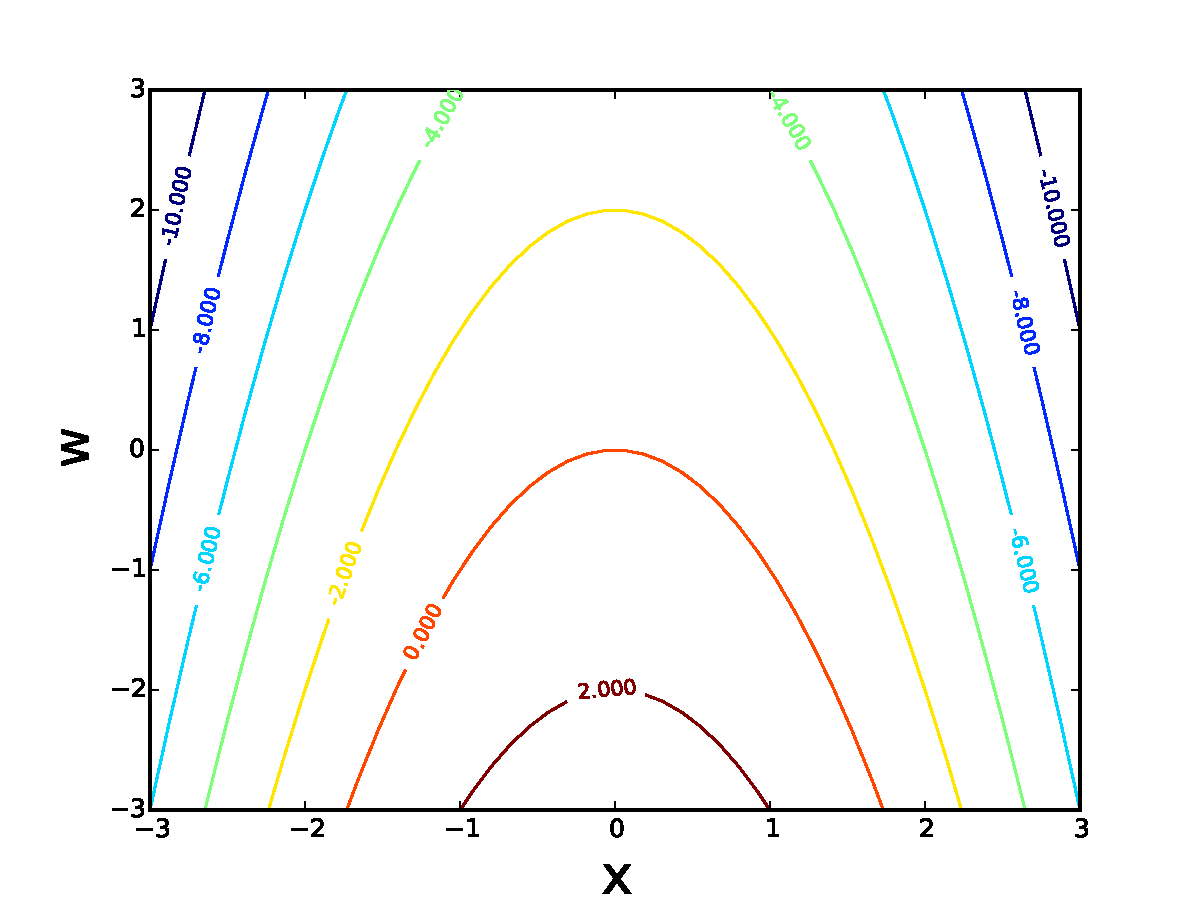
\includegraphics[width=0.44\linewidth]{8F.pdf}}
      \quad
  \subcaptionbox{SBO: The contours of SBO's estimate $\mu_n(x,\w)$ of $F\left(x,\w\right)$, at $n=20$.}[0.45\linewidth]{
      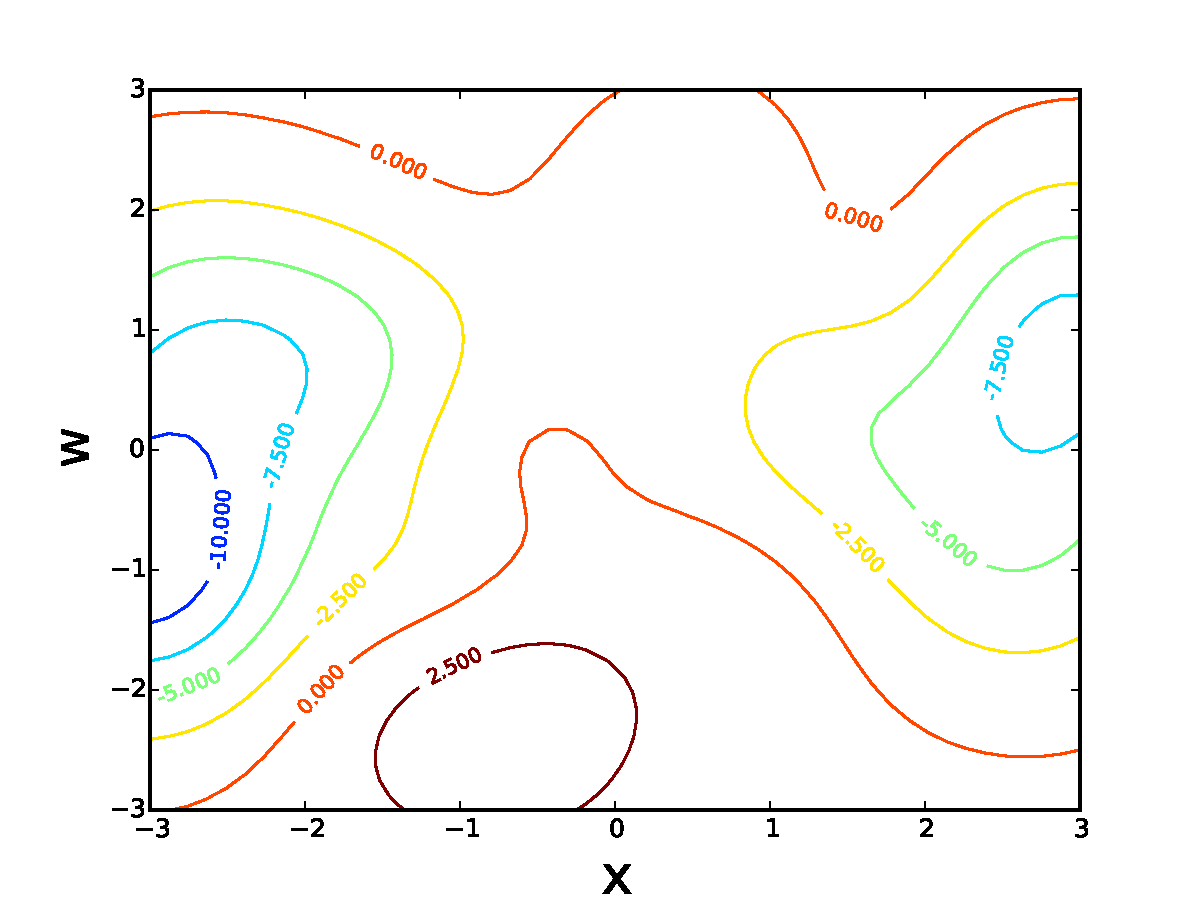
\includegraphics[width=0.44\linewidth]{20muN.pdf}}

  \subcaptionbox{
      SBO: The contours of the value of information $V_n(x,\w)$ under SBO at $n=20$.
  SBO's value of information depends on both $x$ and $\w$.}[0.45\linewidth]{
      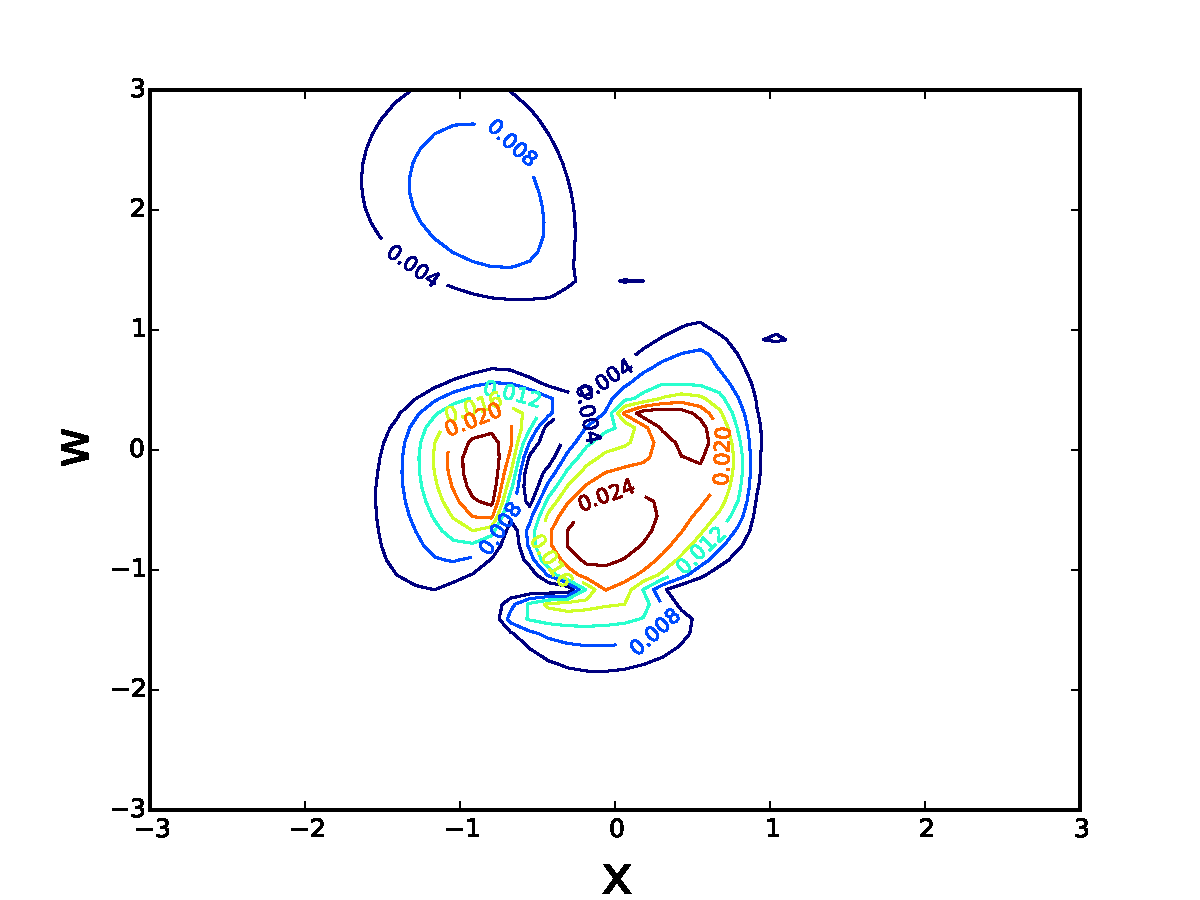
\includegraphics[width=0.44\linewidth]{20VOI.pdf}
  }
  \quad
  \subcaptionbox{
  SBO: The objective $G(x)$, and SBO's estimate $a_n(x)$ and $95\%$ credible interval, at $n=20$.}[0.45\linewidth]{
      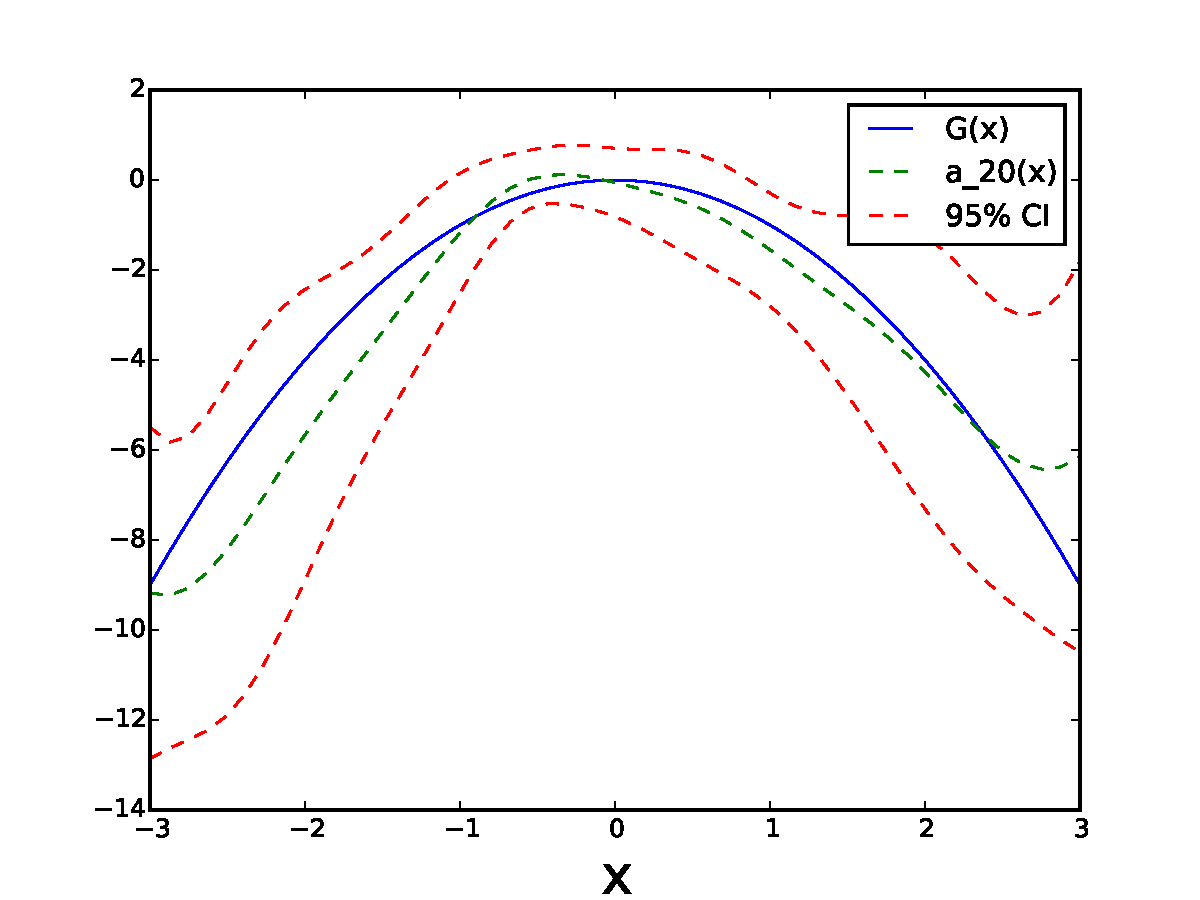
\includegraphics[width=0.44\linewidth]{20a_n.pdf}
  }

  \subcaptionbox{
  KG: The value of information under KG.  KG's value of information depends only on $x$.}[0.45\linewidth]{
      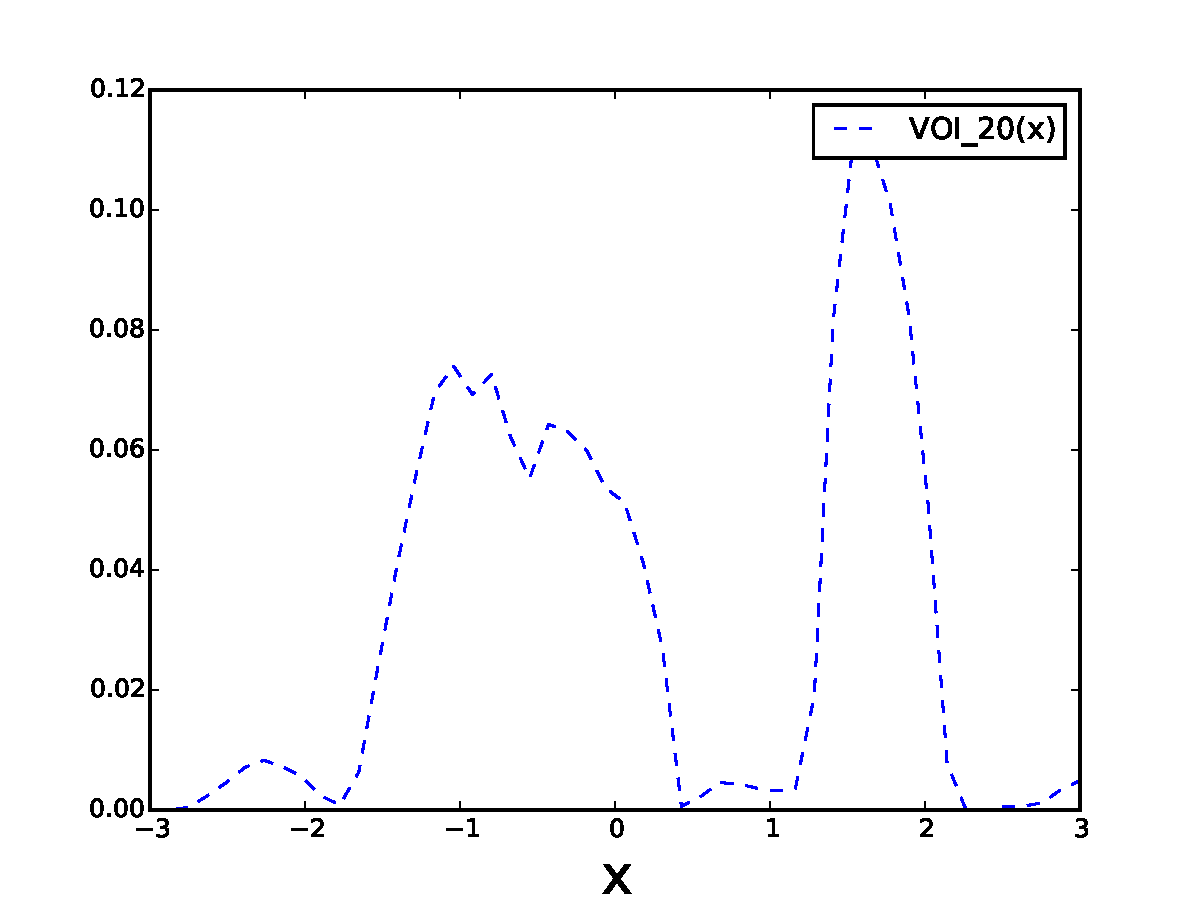
\includegraphics[width=0.44\linewidth]{20VOI_n.pdf}
  }
  \quad
  \subcaptionbox{
  KG: The objective $G(x)$, and KG's estimate $a_n(x)$ and $95\%$ credible interval, at $n=20$.}[0.45\linewidth]{
      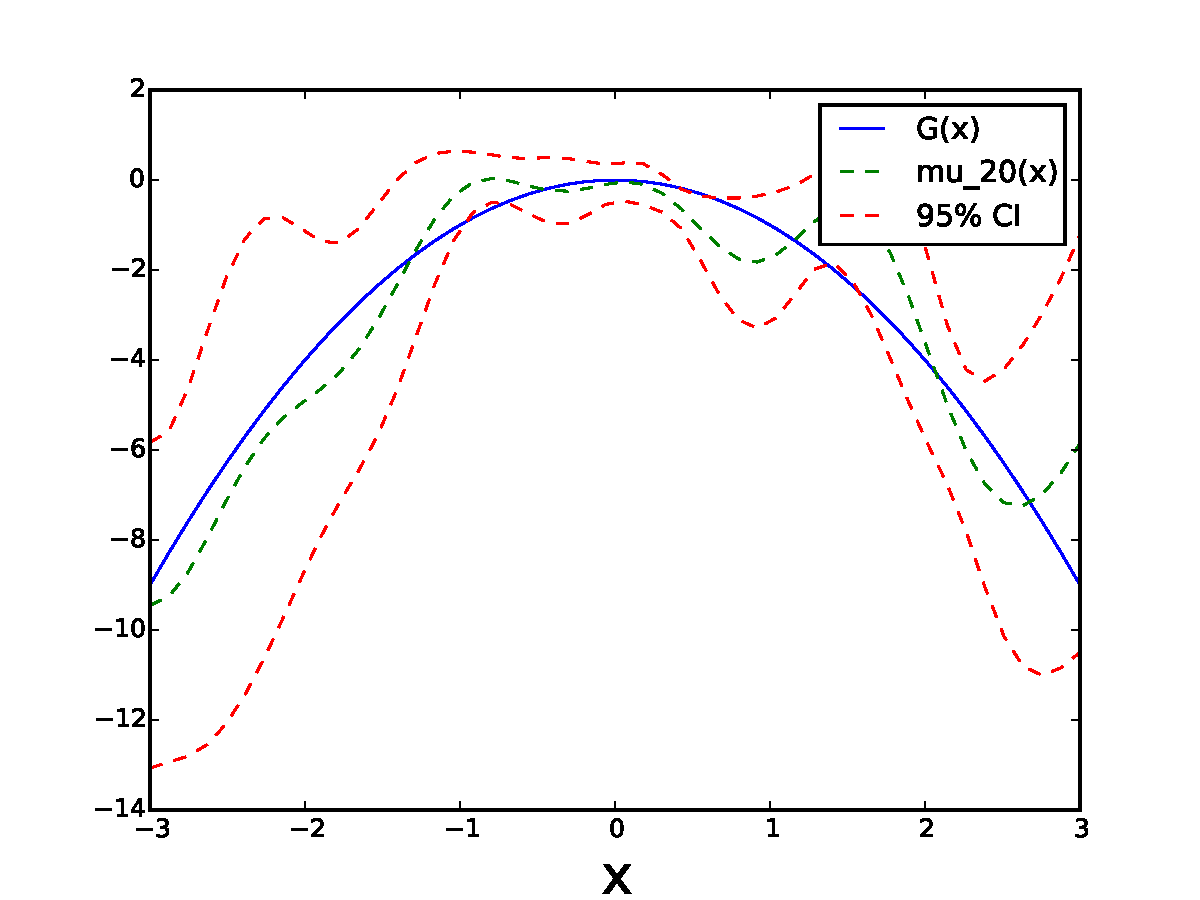
\includegraphics[width=0.44\linewidth]{20mu_n.pdf}
  }
\caption{
    ({\bf First row}) Left shows the contours of $F\left(x,\w\right)=-x^{2}-\w$.  Right shows the contours of SBO's estimate of $F$.  SBO builds a statistical model of $F(x,\w)$, which implies a statistical model on $G(x)$, rather than building a model on $G(x)$ directly like other Bayesian optimization methods.
    ({\bf Second row}) Left shows the contours of SBO's value of information, which depends on both $x$ and $\w$, which SBO uses to choose the pair $(x,\w)$ to sample next.  Right shows SBO's estimates of $G(x)$, which is based on the estimate of $F(x,\w)$ in the first row.
    ({\bf Third row}) Left shows KG's value of information, which depends only on $x$, which KG uses to choose the point $x$ to sample next.  Right shows KG's estimates of $G(x)$.  This estimate is of lower quality than SBO's estimate above, because it does not use the observed values of $\w$.
\label{fig:tahi10}}
\end{figure}

\begin{figure}[!htb]
	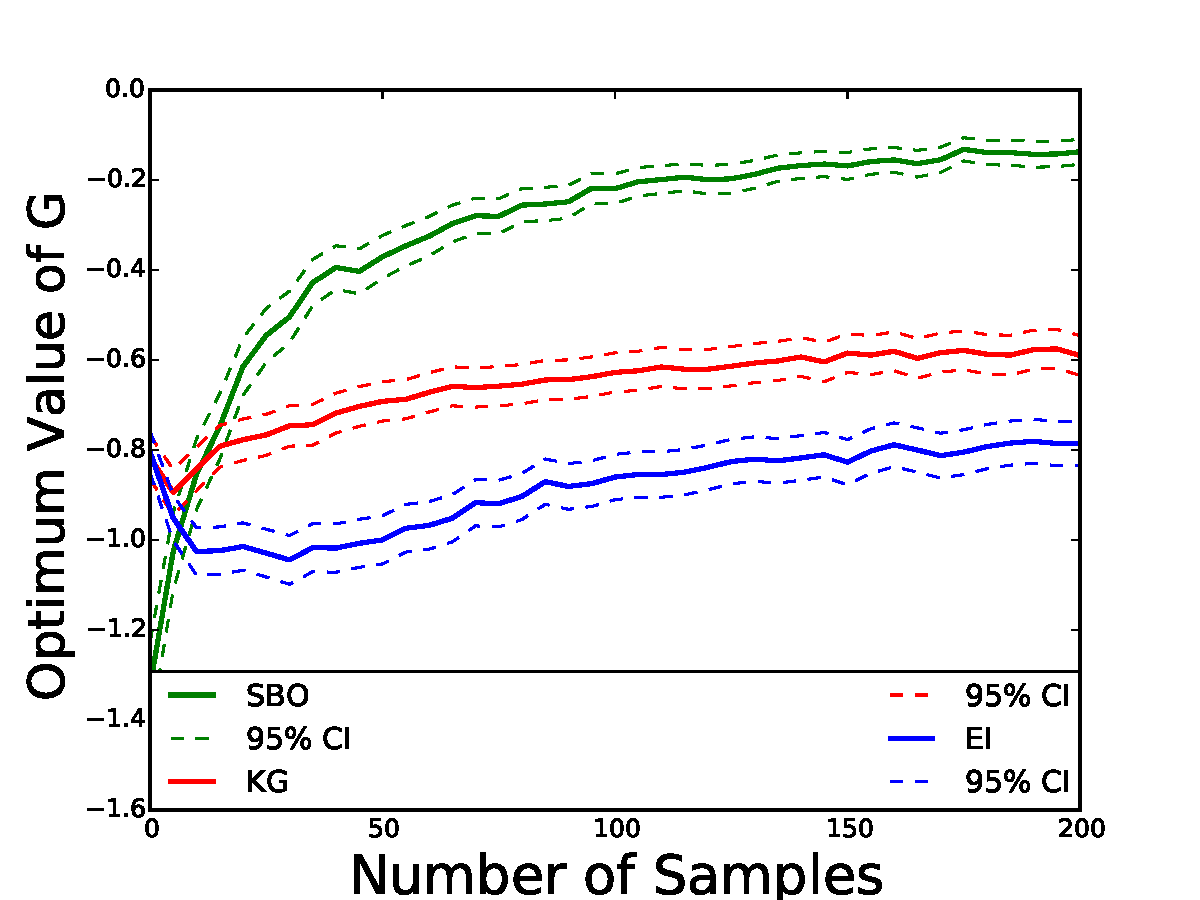
\includegraphics[width=0.9\linewidth]{comparisonSameanal.pdf}
   % \centering
   % \subcaptionbox{Performance comparison between SBO and two Bayesian optimization benchmark, the KG and EI methods, on the analytic test problem from Section~\ref{sec:test} \label{fig:tahi7}}[0.4\linewidth]{
 %   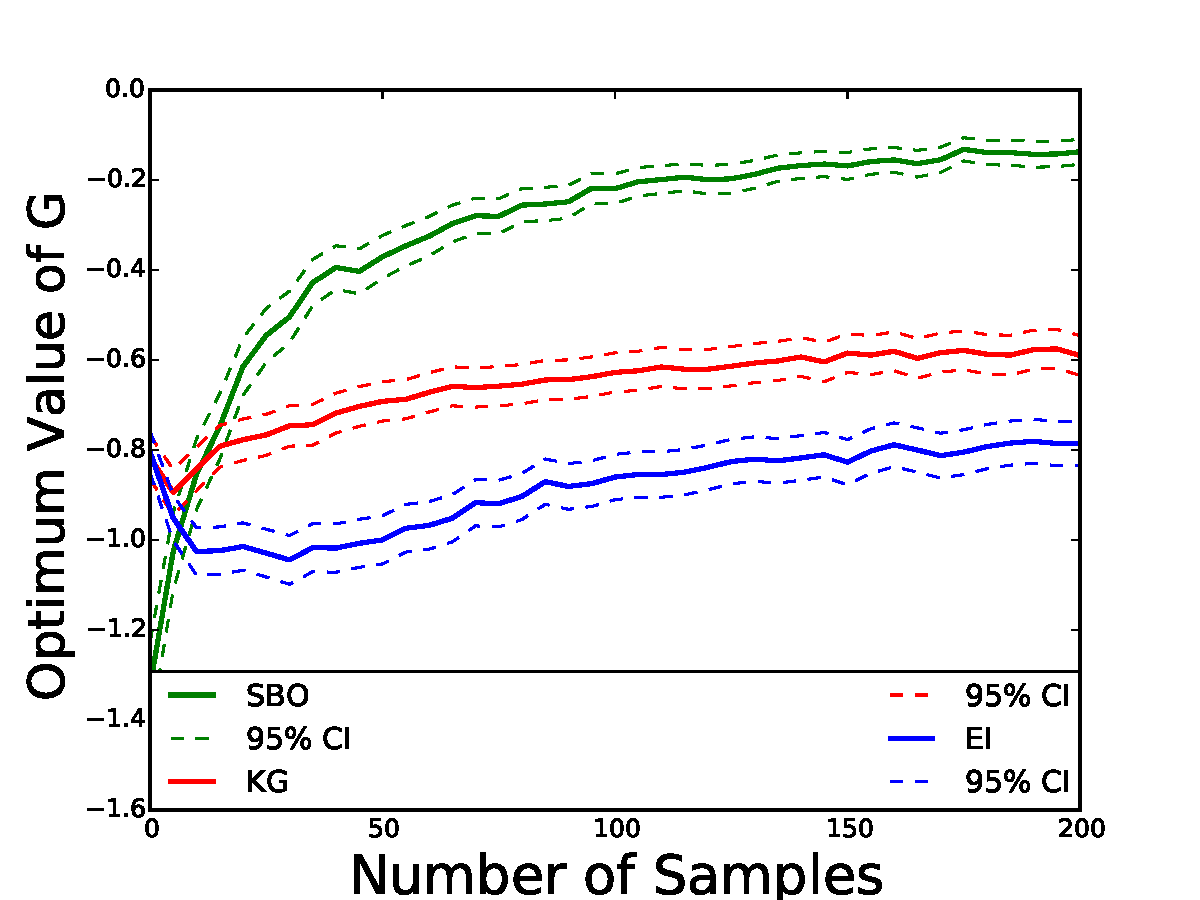
\includegraphics[width=0.4\linewidth]{comparisonSameanal.pdf}}
    \caption{Performance comparison between SBO and two Bayesian optimization benchmark, the KG and EI methods, on the analytic test problem from Section~\ref{sec:test} \label{fig:tahi7}}
\end{figure} 

\subsection{Simulated Problems}
\label{sec:GPexample}

In our next examples, we demonstrate that SBO should be used when the correlation $\mbox{corr}\left[f\left(x,w,z\right),f\left(x,w'z\right)|x,w,w'\right]$ is large enough. We also show that the variance reduction $\frac{\mbox{Var}\left(f\left(x,w,z\right)|x\right)-\mbox{Var}\left(f\left(x,w,z\right)|x,w\right)}{\mbox{Var}\left(f\left(x,w,z\right)|x\right)}$ benefits SBO.
 %the difference of variances $D(x,\w):=\mbox{Var}\left[f\left(x,\w,\z\right)|f,x\right]-\mbox{Var}\left[f\left(x,\w,\z\right)|f,x,\w\right]$ is sufficiently large for many different points $(x,\w)$, or/and% 

We consider the following simulated problems. We define functions $f(x,\w,\z)=h(x,\w)+g(\z)$ on $\left[0,1\right]^{2}\times\mathbb{R}$ where $g(z)$ is drawn from a normal distribution with mean $0$ and variance $\alpha_{d}$, and $h$ is drawn from a Gaussian Process with mean $0$ and and covariance function $\Sigma\left(\left(x,\w\right),\left(x',\w'\right)\right)=\alpha_{h}\exp\left(-\beta\left\Vert \left(x,\w\right)-\left(x',\w'\right)\right\Vert _{2}^{2}\right)$, where $\beta\in\left\{ 2^{-b}:b\in\left\{ -4,-3,-2,-1,0,1,2,3,4,\ldots,15\right\} \right\} $, $\alpha_{h}=\frac{A}{n}$ where $A\in\left\{ \frac{1}{jn}:j\in\left\{ 2,4,8,16\right\} \right\} $ and $n\in\left\{ 1,2,4,8,16\right\} $ is the number of samples taken per iteration, and $\alpha_{d}=\frac{1}{n}-\alpha_{h}$. We also suppose that 
$\w$ is drawn uniformly from $\left\{ 0,1/49,2/49,\ldots,1\right\} $. Consequently, we have that $\mbox{Var}\left[f\left(x,\w,\z\right)|f,x\right]\approx\alpha_{d}+\alpha_{h}=\frac{1}{n}$, $\mbox{Var}\left[f\left(x,\w,\z\right)|f,x,\w\right]\approx\alpha_{d}$, and $\mbox{Cov}\left[f\left(x,\w,\z\right),f\left(x,\w',\z\right)|f,x,z\right]\approx\Sigma\left(\left(x,\w\right),\left(x,\w'\right)\right)$. Consequently,
\begin{align*}
\mbox{corr}\left[f\left(x,w,z\right),f\left(x,w'z\right)|x,w\right]&=\frac{1}{jn-1}\times\\  
&\mbox{exp}\left(-\beta\left\Vert \left(x,w\right)-\left(x,w'\right)\right\Vert _{2}^{2}\right),
\end{align*}

and the variance reduction is equal to

\begin{align*}
\frac{\mbox{Var}\left(f\left(x,w,z\right)|x\right)-\mbox{Var}\left(f\left(x,w,z\right)|x,w\right)}{\mbox{Var}\left(f\left(x,w,z\right)|x\right)}=\frac{1}{jn}.
\end{align*}

We should observe that when $\beta$ is too small or big, the correlation is small. On the other hand, the correlation is large enough if $\beta$ is not too big or small. 

\begin{figure}[!htb]
    \centering
\subcaptionbox{Percentage increase between SBO and a Bayesian optimization benchmark, the KG method, when the variance reduction is $0.5$\label{fig:sim1}}[0.45\linewidth]{
    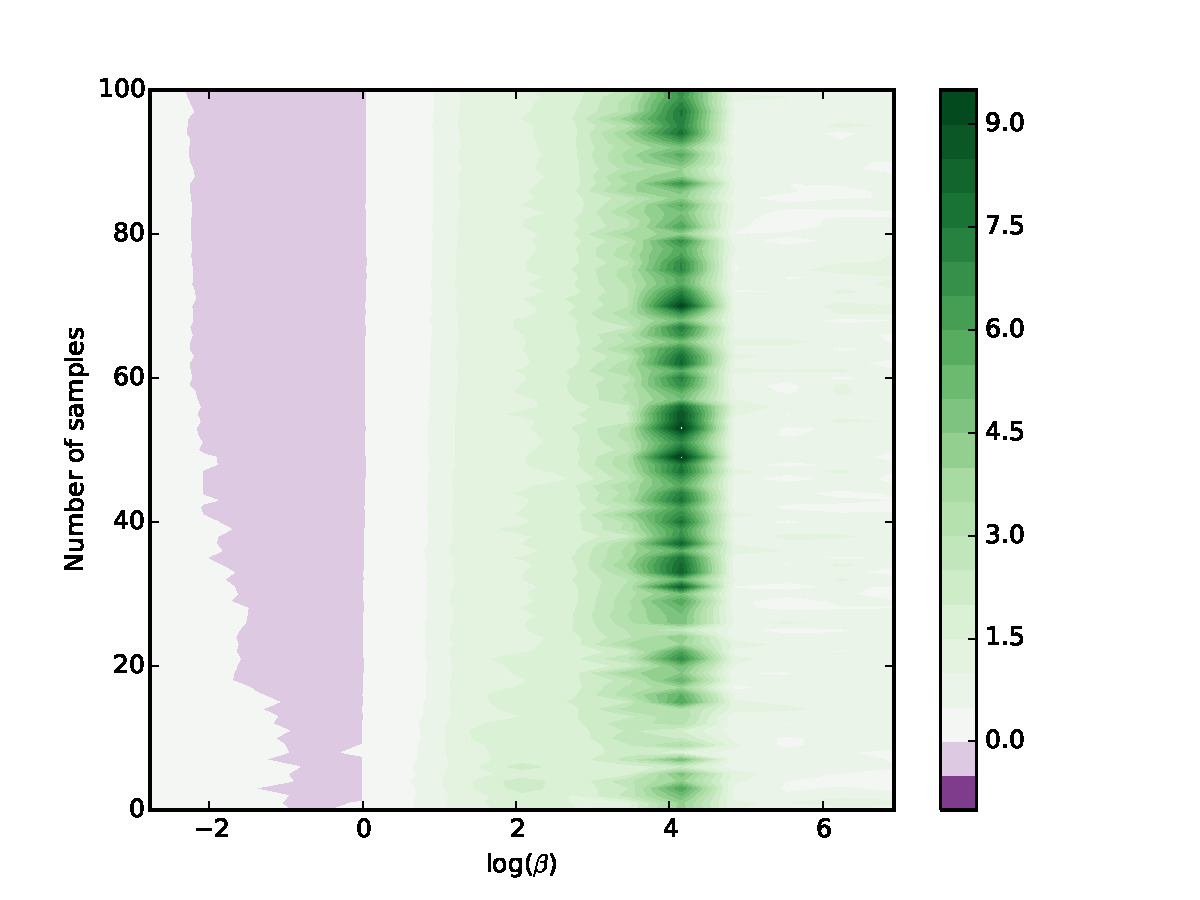
\includegraphics[width=0.45\linewidth]{contourPlotbetahN1A2ver2.pdf}}
    \quad
    \subcaptionbox{Percentage increase between SBO and a Bayesian optimization benchmark, the KG method, when the variance reduction is $1/16$ \label{fig:sim2}}[0.45\linewidth]{
      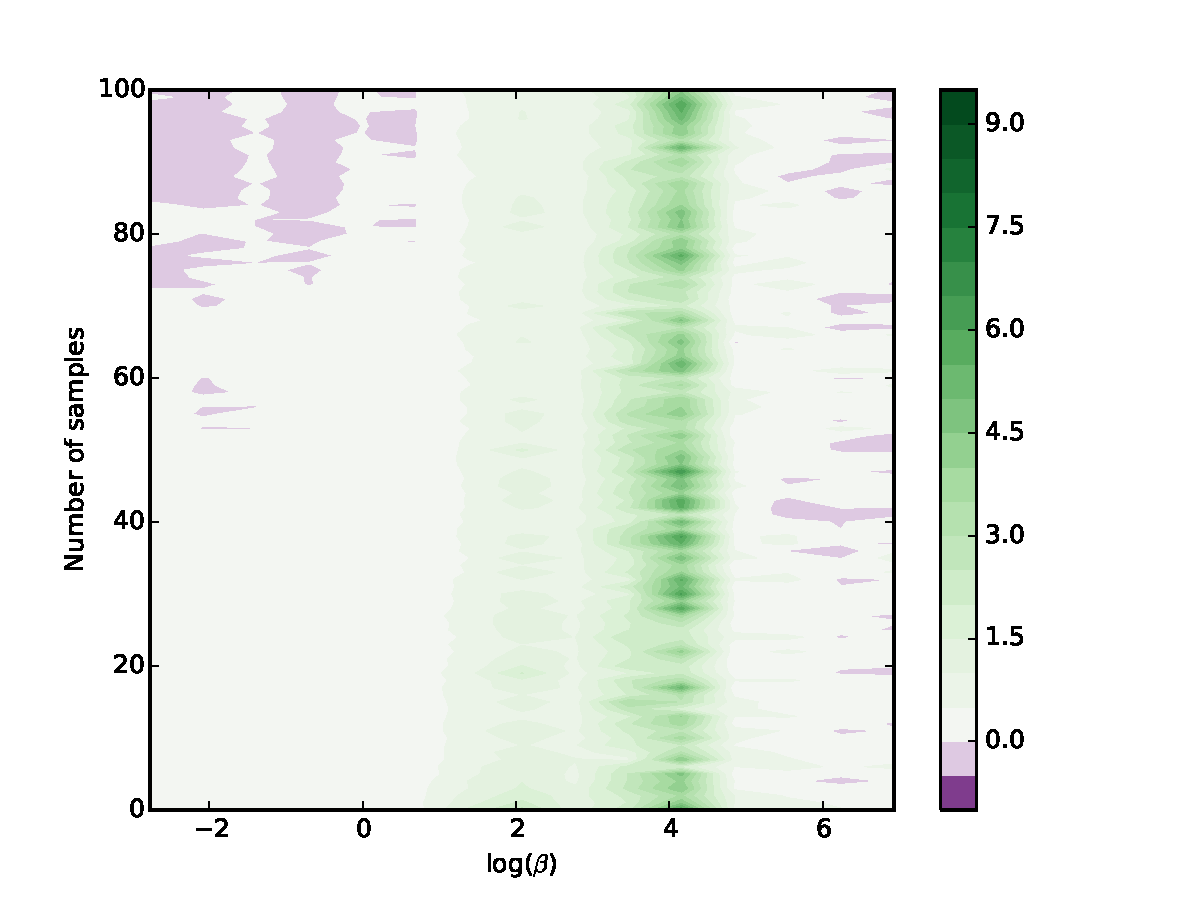
\includegraphics[width=0.45\linewidth]{contourPlotbetahN8A2ver2.pdf}}
\caption{Performance results for SBO on simulated problems when the variance reduction is $0.5$  (plot a), Performance results for SBO on simulated problems when the variance reduction is too small  (plot b).
    \label{fig:simulated}}
\end{figure}

Figure~\ref{fig:sim1} shows percentage increase between SBO and KG when the variance reduction is $0.5$, plotting $\mbox{log}(\beta)$ on the x axis. We see that SBO is always better than KG whenever $\beta >= 1$. Moreover, it is a lot better than KG when $log(\beta)\in(3,5)$. However, KG is slightly better than SBO when $log(\beta)\in(-2,0)$. This essentially means that the correlation benefits SBO, because if $x$ is fixed, then SBO can learn $H(\w)=F\left(x,\w\right)$ for many different $\w$'s when it only evaluates this conditional expectation a few times. We can also see that a large variance reduction is not enough for SBO outperforms KG. 

Figure~\ref{fig:sim2} shows percentage increase between SBO and KG, when the variance reduction is $1/16$. We see that SBO and KG are very similar. However, SBO is again much better when $log(\beta)\in(3.8,4.2)$. We also observe that the variance reduction benefits SBO's performance.

%By doing a factorial analysis, we see that $\beta$ benefits SBO, $A$ benefits KG, there is a positive interaction between $\beta$ and $A$, $n$ and $A$, and a negative interaction between $\beta$, $n$ and $A$, whenever $\beta$ is small enough. 

In conclusion, a large correlation $\mbox{corr}\left[f\left(x,w,z\right),f\left(x,w'z\right)|x,w,w'\right]$ is fundamental, for SBO outperforms KG. A large variance reduction is helpful to improve SBO results, but it is not sufficient.

\subsection{New York City Citi Bike System}
\label{sec:citibike}

In our last example, we consider a queuing simulation based on New York City's Citi Bike system, in which system users may remove an available bike from a station at one location within the city, and ride it to a station with an available dock in some other location within the city.  The optimization problem that we consider is the allocation of a constrained number of bikes (6000) to available docks within the city at the start of rush hour, so as to minimize, in simulation, the expected number of potential trips in which the rider could not find an available bike at their preferred origination station, or could not find an available dock at their preferred destination station.  We call such trips ``negatively affected trips.''

\begin{figure}[!htb]
    \centering
    \subcaptionbox{Performance comparison between SBO and two Bayesian optimization benchmark, the KG and EI methods, on the Citi Bike Problem from Section~\ref{sec:citibike} \label{fig:citibike}}[0.45\linewidth]{
      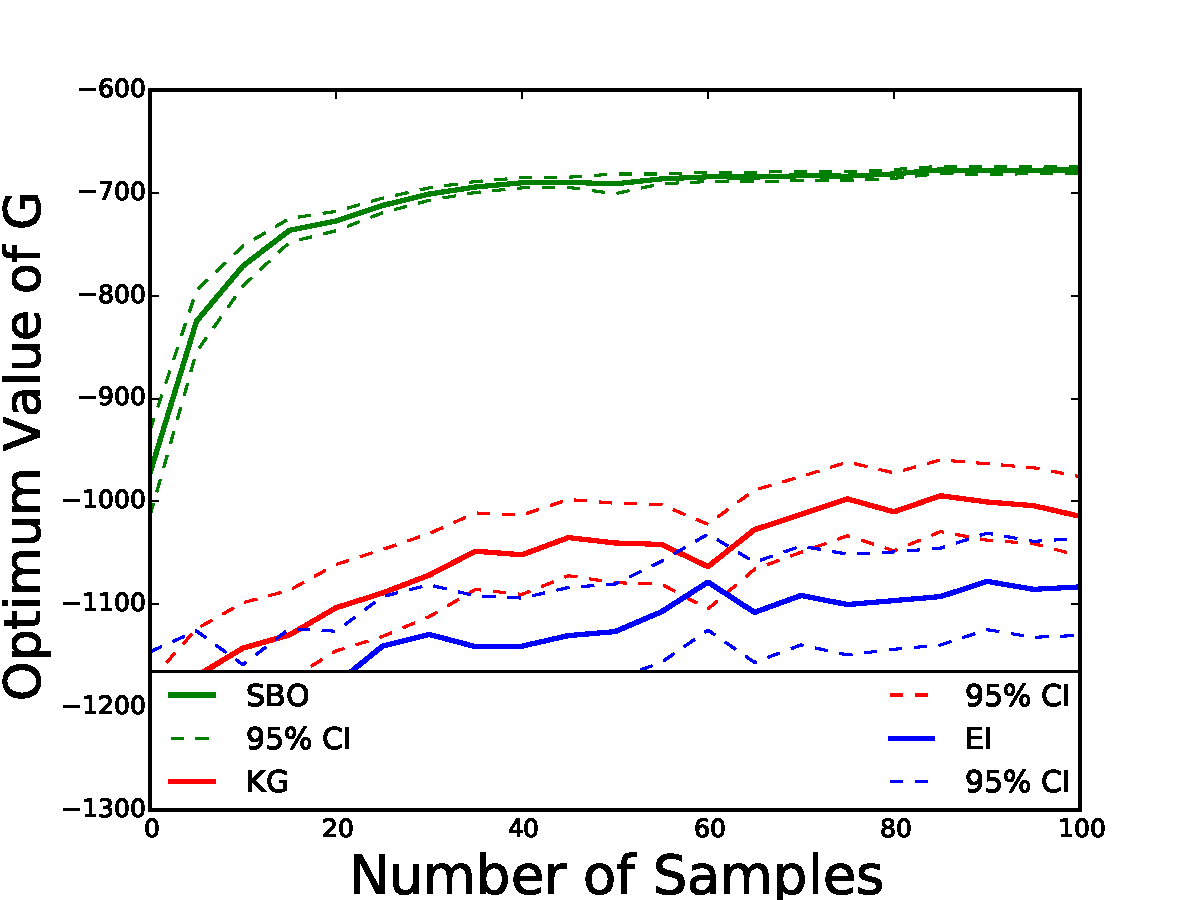
\includegraphics[width=0.45\linewidth]{newcomparisonSameConfiguration.pdf}}
          \quad
     \subcaptionbox{Location of bike stations (circles) in New York City, where size and color represent the ratio of available bikes to available docks.}[0.45\linewidth]{
      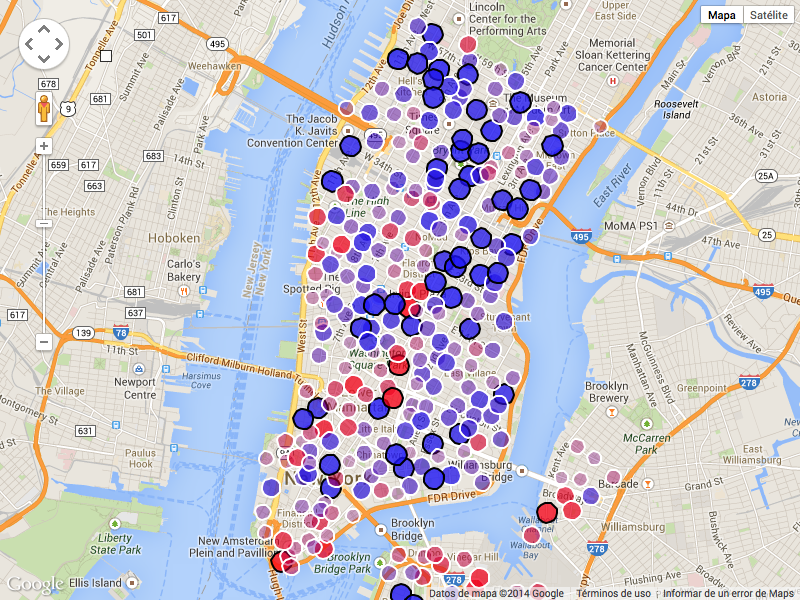
\includegraphics[width=0.45\linewidth]{testStationMapPng0-full.png}}
\caption{Performance results for the Citi Bike problem (plot 1), and a screenshot from our simulation of the Citi Bike problem (plot b).
    \label{fig:stuff}}
\end{figure}

% In the last example, we simulated bike usage on the morning rush hours for New York City's bike sharing system. A bike sharing system is a group of bikes placed in different bike stations. People can rent these bikes and return them to any bike station after usage. 

We simulated in Python the demand of bike trips of a New York City's Bike System on any day from January 1st to December 30th between 7:00am and 11:00am. We used 329 actual bike stations, locations, and numbers of docks from the Citi Bike system, and estimated demand and average time for trips for every day in a year using publicly available data of the year 2014 from Citi Bike's website \cite{citibike}.

% This dataset  contains start bike station, end bike station, station latitude and longitude, and trip time for each bike trip. We considered $329$ bike stations and $600$ bikes. 

We simulate the demand for trips between each pair of bike stations on a day using an independent Poisson process, and trip times between pairs of stations follows an exponential distribution. 
If a potential trip's origination station has no available bikes, then that trip does not occur, and we increment our count of negatively affected trips.  If a trip does occur, and its preferred destination station does not have an available dock, then we also increment our count of negatively affected trips, and the bike is returned to the closest bike station with available docks.

We divided the bike stations in $4$ groups using k-nearest neighbors, and let $x$ be the number of bikes in each group at 7:00 AM. We suppose that bikes are allocated uniformly among stations within a single group.  Then we consider a directed graph between the bike stations, where each pair of bike stations has two directed edges, and we divided these edges in $4$ groups. If the edge $(i,j)$ is in a group, then $(j,i)$ is also in that group. The random variable $\w$ is the total demand of bike trips during the period of our simulation. The random vector $\z$ contains all other random quantities within our simulation.

We provide a table with concrete mapping of the SBO abstractions onto the CitiBike example,
\begin{table}[htbp]
\caption{Table of Notation.}
\label{table}
\centering
\begin{center}
\begin{small}
\begin{tabular}{lrp{5.5cm}}
\hline
$x\in\mathbb{R}^{4}$ & $\triangleq$ & deterministic vector that represents the number of bikes in each group of bike stations at 7:00 AM.\\
$\w\in\mathbb{N}$ & $\triangleq$ & Poisson random variable that represents the total demand of bike trips between 7:00am to 11:00am\\
$\z$ & $\triangleq$ & Random vector that consists of: i) day of the year where the simulation occurs, ii) $\binom{329}{2}$-dimensional Poisson random vector that represents the total demand between each pair of bike stations, iii) exponential random vector that represents the time duration of each bike trip. \\
$-f(x,\w,\z)$ & $\triangleq$ & negatively affected trips between 7:00am to 11:00am.\\
$G(x)$ & $\triangleq$ & $\mathbb{E}[f(x,\w,\z)]$. \\
\end{tabular}
\end{small}
\end{center}
\end{table}

Figure~\ref{fig:citibike} compares the performance of SBO, KG and EI, plotting the number of samples beyond the first stage on the $x$ axis, and the average true quality of the solutions provided, $G(\mathrm{argmax}_x \mathbb{E}_n[G(x)])$, averaging over 300 independent runs of the three algorithms. We see that SBO was able to quickly find an allocation of bikes to groups that attains a small expected number of negatively affected trips. 


% We estimated the parameters of the simulation using the data available at Citi Bike's website\footnote{https://www.citibikenyc.com/}. This dataset  contains start bike station, end bike station, station latitude and longitude, and trip time for each bike trip. We considered $329$ bike stations and $600$ bikes. 

%\begin{figure}[htp]
%\centering
%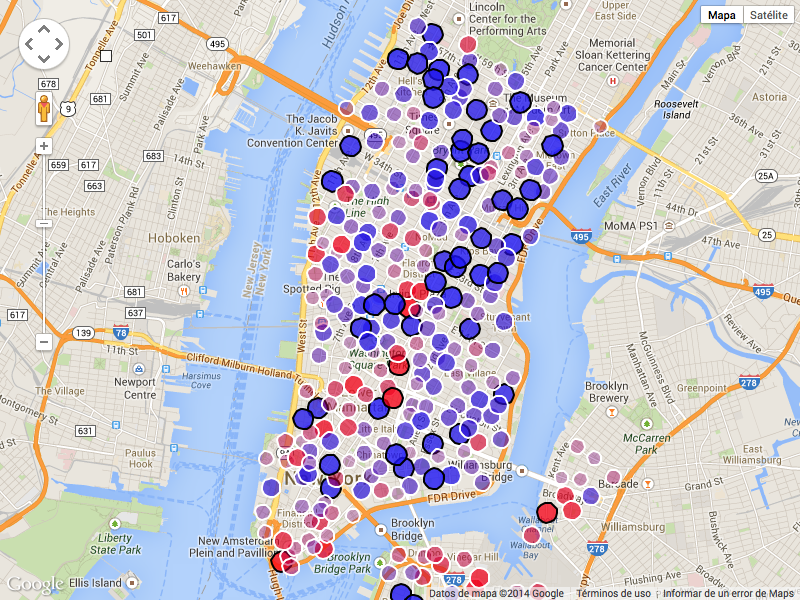
\includegraphics[width=.5\textwidth]{testStationMapPng0-full.png}
%%\caption{Circles are the different bike stations in New York City. The size and color represents the ratio of available bikes to available docks. If the color is blue, this ratio is "big", and it is red otherwise.}
%\label{example2}
%\end{figure}



\section{Conclusion}
\label{conclusion}
We have presented a new algorithm called SBO for simulation optimization of noisy derivative-free expensive functions. This algorithm can be used with high dimensional random vectors, and it also outperforms the classical Bayesian approach to optimize functions in the examples presented. 


% Acknowledgements should only appear in the accepted version. 
\section*{Acknowledgements} 
 
\textbf{Do not} include acknowledgements in the initial version of
the paper submitted for blind review.

% In the unusual situation where you want a paper to appear in the
% references without citing it in the main text, use \nocite
\nocite{langley00}

\bibliography{example_paper}
\bibliographystyle{icml2016}

\end{document} 


% This document was modified from the file originally made available by
% Pat Langley and Andrea Danyluk for ICML-2K. This version was
% created by Lise Getoor and Tobias Scheffer, it was slightly modified  
% from the 2010 version by Thorsten Joachims & Johannes Fuernkranz, 
% slightly modified from the 2009 version by Kiri Wagstaff and 
% Sam Roweis's 2008 version, which is slightly modified from 
% Prasad Tadepalli's 2007 version which is a lightly 
% changed version of the previous year's version by Andrew Moore, 
% which was in turn edited from those of Kristian Kersting and 
% Codrina Lauth. Alex Smola contributed to the algorithmic style files.  
